\section{Frozen-policy performance and opponent dependence}
\label{sec:jesper-results}
\contributionauthor{Jesper Eggers}
Table~\ref{tab:jesper-frozen-evaluation} reports all eight evaluated
configuration--opponent combinations, with 200 games each. The native
final policy scores 1.945 points per game against three rule-based
opponents, with a 95\% interval of [1.655, 2.250]. Its mean comprises
1.295 coins and 0.130 credited kills; multiplying the latter by five
accounts for the remaining 0.650 points. Survival is 45.0\%, while
self-destruction occurs in 54.0\% of games. Of 110 deaths, 108 include
self-destruction credit, identifying frequent exposure to the agent's own blasts.
Repeated bombing and a strong safety diagnostic do
not by themselves establish a strong competitive player.

Against the mixed population, native mean score rises to 2.640
[2.285, 3.015], comprising 1.415 coins and 0.245 kills. The 0.695-point
difference from the rule-based population consists of 0.120 additional
coin points and 0.575 additional kill points. This decomposition identifies
the source of the observed score change, without attributing it to an
unmeasured learning mechanism. Survival rises to 51.5\% and self-destruction
falls to 44.0\%. These are results for one frozen artifact facing two
specified populations, rather than a universal measure of opponent
difficulty.

Relative rank gives a different perspective. The native agent's tie-aware
score-leader share is 15.4\% [10.8, 20.2] against three rule-based opponents
and 10.2\% [6.5, 14.5] against the mixed population. The higher absolute
score in mixed games therefore does not translate into a higher observed
share of first places. Changing opponents also changes the scores the
focal agent must exceed. This rank comparison is descriptive; the paired
component tests are conducted within each population. The results show why
official return and relative success should both be reported.

\begin{table}[htbp]
\centering\footnotesize
\setlength{\tabcolsep}{3pt}
\begin{tabularx}{\textwidth}{@{}Yrrrrrrr@{}}
\toprule
Configuration & Games & Score [95\% CI] & Coins & Kills & \shortstack{Self-\\destruction (\%)} & \shortstack{Survived\\(\%)} & \shortstack{Leader\\share (\%)} \\
\midrule
\multicolumn{8}{@{}l}{\textit{Three rule-based opponents}} \\
Final Q + temporal mask & 200 & 1.95 [1.66, 2.25] & 1.295 & 0.130 & 54.0 & 45.0 & 15.4 \\
Final Q + RUEHL mask & 200 & 0.57 [0.42, 0.73] & 0.520 & 0.010 & 90.5 & 3.0 & 2.4 \\
Random + temporal mask & 200 & 1.09 [0.85, 1.34] & 0.590 & 0.100 & 43.0 & 43.5 & 5.4 \\
Random + RUEHL mask & 200 & 0.15 [0.10, 0.21] & 0.150 & 0.000 & 97.0 & 0.5 & 0.0$^{\dagger}$ \\
\addlinespace
\multicolumn{8}{@{}l}{\textit{Mixed opponent population}} \\
Final Q + temporal mask & 200 & 2.64 [2.29, 3.02] & 1.415 & 0.245 & 44.0 & 51.5 & 10.2 \\
Final Q + RUEHL mask & 200 & 0.51 [0.39, 0.64] & 0.480 & 0.005 & 98.0 & 1.0 & 0.5 \\
Random + temporal mask & 200 & 1.14 [0.91, 1.39] & 0.665 & 0.095 & 31.5 & 63.0 & 2.0 \\
Random + RUEHL mask & 200 & 0.15 [0.10, 0.21] & 0.155 & 0.000 & 98.5 & 0.0 & 0.0$^{\dagger}$ \\
\addlinespace
\bottomrule
\end{tabularx}
\caption{Episode means from 200 games per row; score brackets are 95\% episode-bootstrap intervals. Other columns are point estimates, with intervals retained in the supplementary JSON. Score-leader share splits credit among tied highest final scores, including dead agents. Inference is conditional on one checkpoint and the stated opponents. $^{\dagger}$The degenerate all-zero bootstrap interval is suppressed; zero score-leading episodes among 200 games gives a Wilson upper bound of 1.9\% on leader presence, which also bounds expected fractional share.}
\label{tab:jesper-frozen-evaluation}
\end{table}


With the same temporal mask, random selection scores 1.090 against
rule-based opponents and 1.140 against the mixed population. Learned
ranking adds 0.855 points [0.490, 1.220] and 1.500 points [1.080, 1.920],
respectively, in paired comparisons. For rule-based opponents, 0.705
of the advantage comes from coins and 0.150 from kills. In mixed games,
coins and kills contribute 0.750 points each. The improvement is therefore
measurable beyond the hand-designed constraints, with its composition
depending on the opponents.

Higher score does not imply lower risk. Learned temporal selection
increases self-destruction over its random control by 11.0 percentage
points [2.0, 20.5] against rule-based opponents and 12.5 percentage points [3.5, 21.5]
in mixed games. Its mixed-game survival decreases by 11.5 percentage points
[2.5, 20.5]. The trained ordering is more productive under the official
score while retaining a substantial safety weakness. Choosing a policy
solely from survival would miss its scoring benefit; choosing solely
from score would conceal the remaining self-inflicted losses.

\begin{figure}[!htbp]
\centering
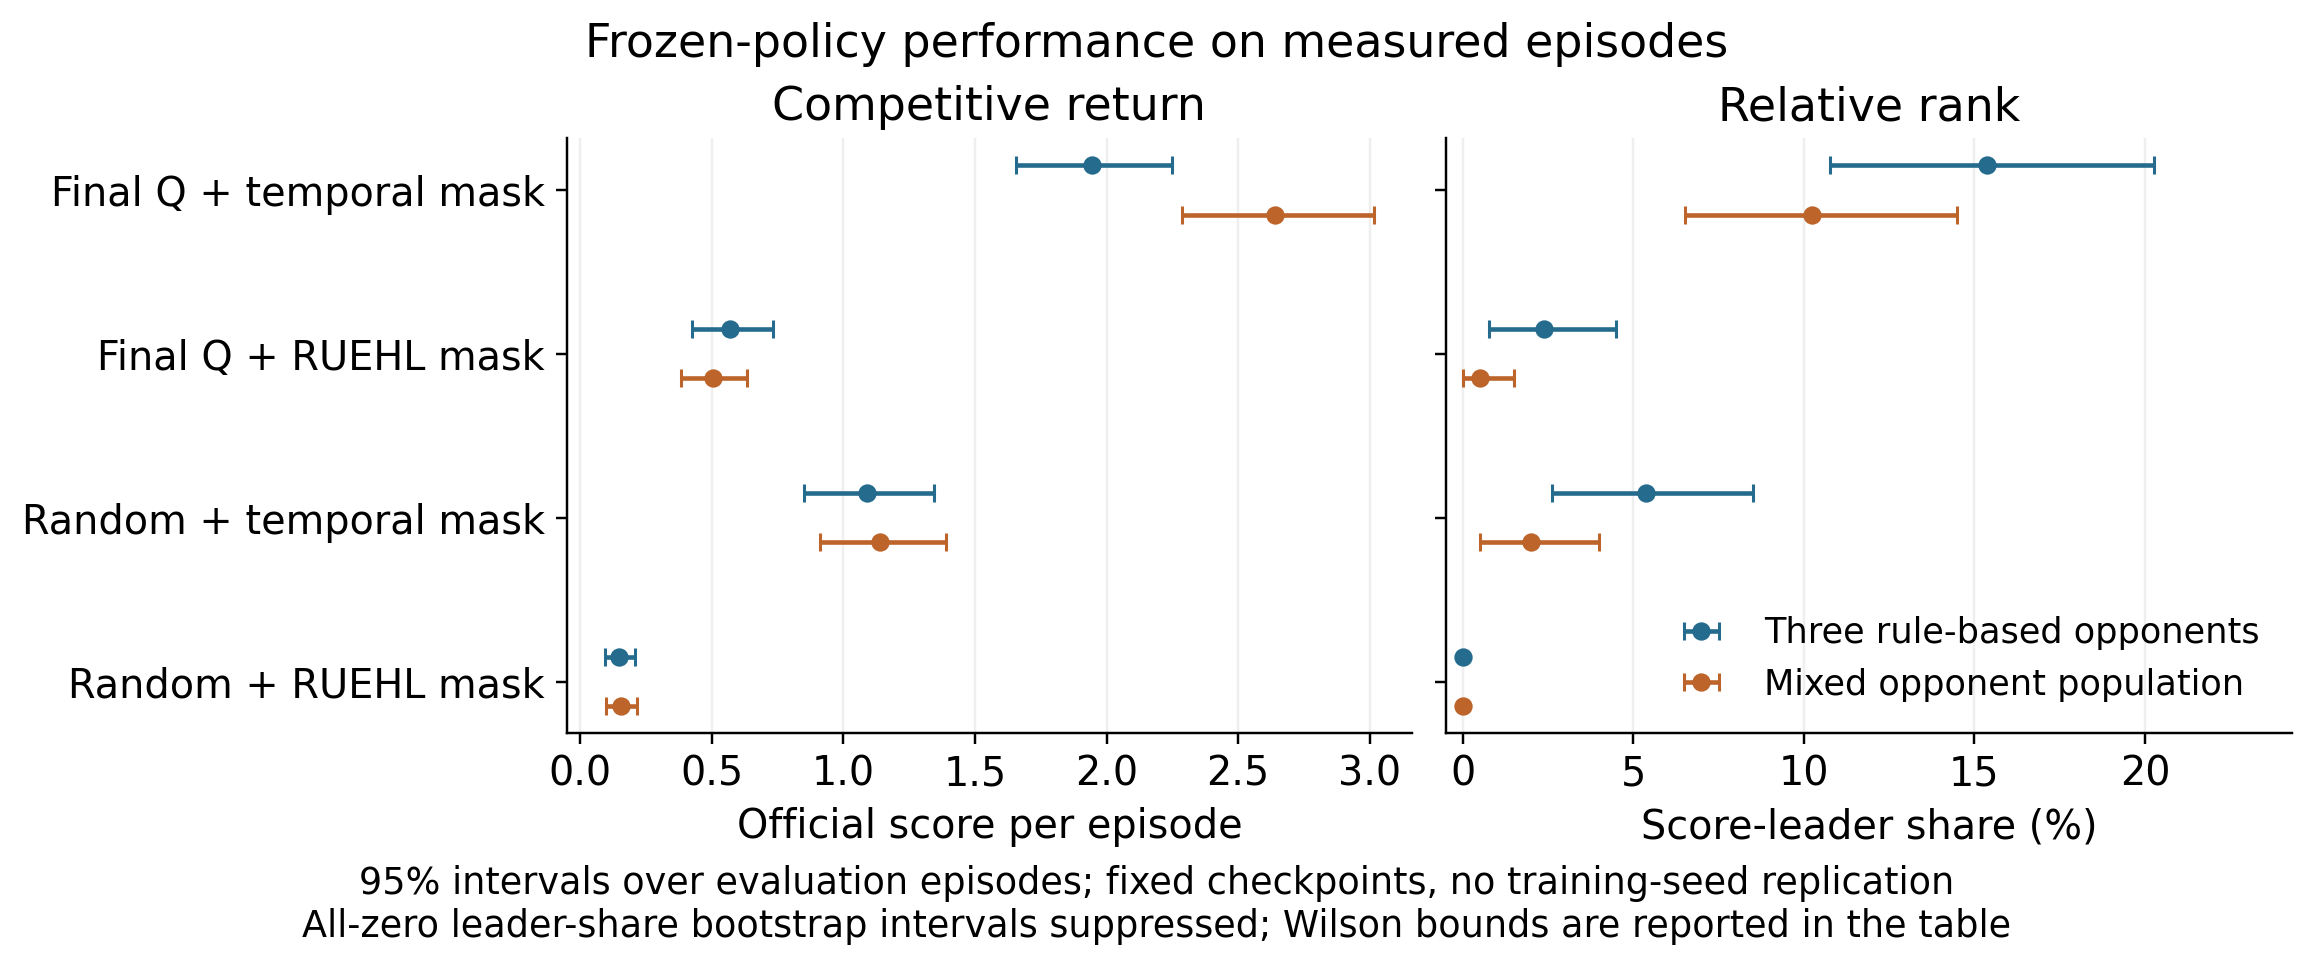
\includegraphics[width=\textwidth]{figures/frozen_evaluation_performance.png}
\caption{Official return and score-leader share for the four frozen
decision configurations and two opponent populations. All learned rows
use the same final-network weights.}
\label{fig:jesper-performance}
\end{figure}
\FloatBarrier
